\documentclass[student]{ITRslides}
\usepackage{tikz,pgfplots,epstopdf,psfrag,pstricks,mathtools}
\pgfplotsset{compat=1.9}
\usepgfplotslibrary{groupplots}
\usetikzlibrary{matrix} 
\addbibresource{MyCollection.bib}
%\AtEveryBibitem{\clearfield{note}}
\AtEveryBibitem{\clearfield{isbn}}
\AtEveryBibitem{\clearfield{doi}}
\AtEveryBibitem{\clearfield{issn}}
\AtEveryBibitem{\clearname{editor}}
\graphicspath{{pics/}{logos/}}
\newcommand{\f}[1]{\boldsymbol{#1}}
\newcommand{\g}[1]{\text{#1}}

\title{Human behaviour modelling for teleoperation}
\presenter{M. Angerer}

\supervisor{S. Musi\'c}
\typeofpres{Advanced Seminar}

\usetikzlibrary{decorations.pathreplacing}
\newcommand{\tikzmark}[2]{\tikz[remember picture,baseline=(#1.base)]{\node[inner sep=0pt] (#1) {#2};}}


%%%%%%%%%%%%%%%%%%%%%%%%%%%%%%%%%%%%%%%%%%%%%%%%%%%%%%%%%%%%%%%%%%%%%%%%%%%%%%%%

\begin{document}


\begin{frame}
    \titlepage
\end{frame}

%\begin{frame}
%	\frametitle{Overview}
%    \tableofcontents%[hideallsubsections]%[pausesections]
%\end{frame}

\section{Introduction}

\begin{frame}
	\frametitle{Human roles in teleoperation}


			\begin{figure}
			
			%\psfrag{q1}[Bl][Bl]{\small $\alpha$}
			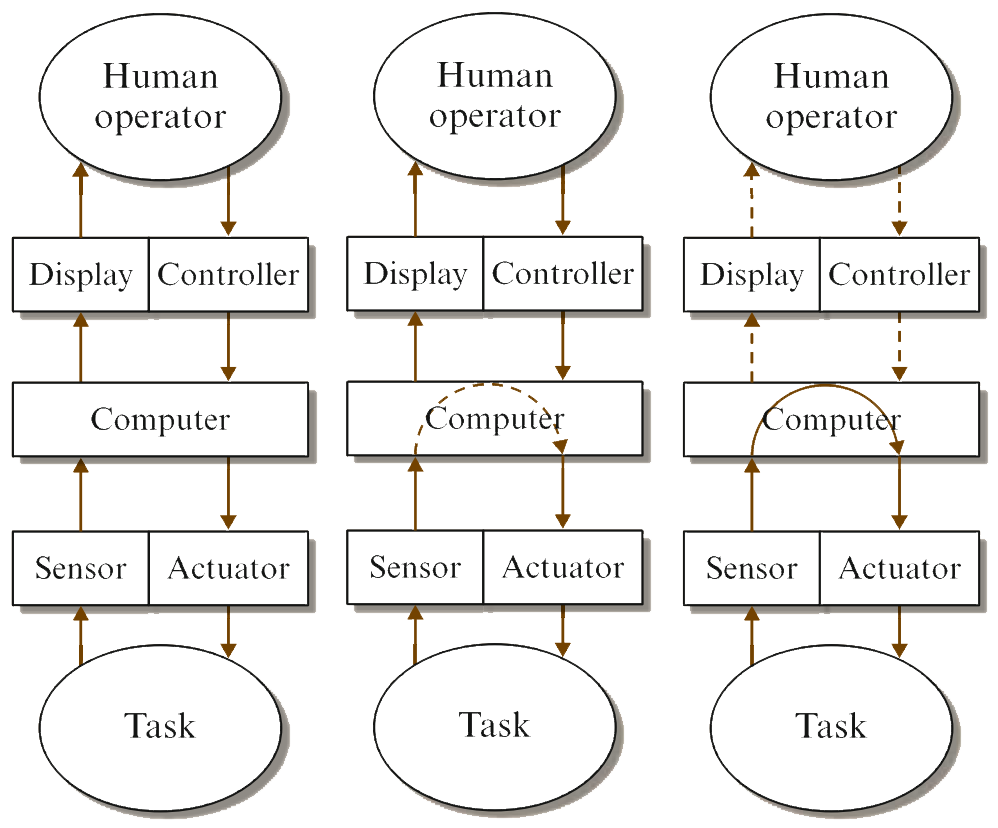
\includegraphics[width=0.7\textwidth]{DirectSharedSup.png}
			%\scriptsize{Coordinated use of tools: Pipe cutting}\nocite{MHI-MEISTeR}{\tiny{ [MHI14]}} 
			\end{figure}
		\vspace{-20pt}
\begin{center}
 Direct \hspace{14mm} Shared \hspace{10mm} Supervisory
\end{center}
 
		
			

\end{frame}

\begin{frame}
	\frametitle{Sensory perception, Cognition \& Response}
	General classification of behavioural activity \nocite{Sheridian1992}{\tiny [She92]}
	\begin{itemize}
	\item Sensory perception modelling \\
	 	... determines the usefulness of provided information
	\item Cognitive modelling \\
		... what a human \emph{will} do in a certain situation
	\item Response or motor function modelling \\
		... what a human \emph{can} do, physiological limits apply
	\end{itemize}
		
	
	

\vspace{6pt}
{\color{tum_blue}\textbf{Human modelling in teleoperation can}}\vspace{-6pt}
\noindent{\color{tum_blue}\rule[0.5ex]{\linewidth}{1.5pt}}
	\begin{itemize}
	\item ensure stability with the human in the loop
	\item support decision making 
	\item improve manipulation skill
	\end{itemize}


\end{frame}

%\begin{frame}
%	\frametitle{Related Work}
%	\textbf{Low-level coordination}
%	\begin{itemize}
%		\item (Inverse) grasp-matrix approaches \nocite{Schneider_92,Caccavale_08} {\tiny [SC92,CCMV08]} 	
%		\item Virtual structures \nocite{Stramigioli_01, Sieber_15} {\tiny [Str01,SMH15]} 
%	\end{itemize}
%	\textbf{Human in the loop}
%	\begin{itemize}	
%		\item Bilateral tele-manipulation  \nocite{Lee_05} {\tiny [LS05]} 	
%		\item Human leader - robotic followers \nocite{Sieber_15, Scheggi_14}{\tiny [SMH15,SMP14]} 
%		\item Gesture-based Control \nocite{Gioioso_2014}{\tiny [GFS+14]} 
%	\end{itemize}
%	\textbf{Safety by energy-regulation}
%	\begin{itemize}
%		\item Adaptive impedance control of a single manipulator \nocite{Tadele_14}{\tiny [TVS14]}
%		\item Energy observer in physical human-robot interaction \nocite{Geravand_16}{\tiny [GSLP16]}
%	\end{itemize}
		
%			\begin{block}{}
%
%\hspace*{1mm} Stability with non-restrictive input interfaces is unexplored \\
% \hspace*{1mm} Passivity is commonly used to cope with unmodelled dynamics \\
% \hspace*{1mm} Energy-based safety metrics apply for impact limitation 
%
%			\end{block}
			
%			\vspace{6pt}
%			{\color{tum_blue}\textbf{Conclusion}\vspace{-6pt}
%			\noindent\rule[0.5ex]{\linewidth}{1.5pt}}
%			\begin{itemize}
%				\item Stability with non-restrictive input interfaces is unexplored
%				\item Passivity is commonly used to cope with unmodelled dynamics
%				\item Energy-based safety metrics apply for impact limitation
%			\end{itemize}
%\end{frame}

%\begin{frame}
%	\frametitle{Related Work: Human in the loop}
%	\begin{itemize}	
%		\item Formation-based control \nocite{Sieber_15, Scheggi_14}{\tiny [SMH15,SMP14]} 
%%		\begin{itemize}
%%			\item Single leader, multiple followers
%%			\item Robots preserve formation autonomously
%%			\item Tactile feedback
%%		\end{itemize}
%		\item Bilateral tele-manipulation  \nocite{Lee_05} {\tiny [LS05]} 
%%		\begin{itemize}
%%			\item Single master coupled to human, constrained system as slave
%%			\item Local control of interaction dynamics
%%			\item Force feedback
%%		\end{itemize}
%
%		\item Gesture-based Control \nocite{Gioioso_2014}{\tiny [GFS+14]} 
%%		\begin{itemize}
%%			\item Free-hand motion controls constrained system
%%			\item Visual feedback
%%			%\item only visual feedback
%%		\end{itemize}
%		\end{itemize}
%		
%			\begin{block}{}
%			\begin{itemize}
%			\item port-Hamiltonian systems allow for energy consistent modelling of complex physical systems
%			\item \emph{IPC} concept based on a physical model
%
%			\item Closed loop stability for bounded energy supply% and a passive control architecture
%			\end{itemize}
%
%	\end{block}
%	
%\end{frame}

\section{Actuation}

%\begin{frame}
%	\frametitle{port-Hamiltonian systems}
%\emph{Hamiltonian} equations of a mechanical system
%\[ \dot{q} = \frac{\partial H}{\partial p}(q,p) \]
%\[\dot{p} = -\frac{\partial H}{\partial q}(q,p) + F \]
%\emph{Hamiltonian} $ H(q,p)$: total energy\\
%generalized coordinates $q$, generalized momenta $p$, external generalized forces $F$
% 
%\textbf{Energy balance}
%\[ \frac{d}{dt} H = \frac{\partial^T H}{\partial q} \dot{q} + \frac{\partial^T H}{\partial p}\dot{p} = \frac{\partial^T H}{\partial p} F = \dot{q}^T F \]
%
%\end{frame}


%\begin{frame}
%	\frametitle{Overall control architecture}
%	
%	\begin{figure}
%		\centering
%		%\psfrag{q1}[Bl][Bl]{\small $\alpha$}
%		\def\svgwidth{0.99\columnwidth}
%		\input{pics/overview.eps_tex}
%	\end{figure}
%	\begin{itemize}
%		\item Source for the robot-team controller: Energy Tank
%		\item Human user controls the power flow
%		\item Energy supplied to the robots is re-supplied to the tank
%	\end{itemize}
%	\begin{block}{}
%		Energy-consistent description in the \emph{port-Hamiltonian} framework
%		\end{block}
%	
%\end{frame}


\begin{frame}
	\frametitle{Bilateral telemanipualtion}
	Haptic interface with force feedback: Human is an impedance\\
	Delayed communication line: Wave transformation distorts displayed environment\\   
		System identification: human motion is inherently dissipative \nocite{Rahman1999}{\tiny [RIM99]}\\
		 A dissipative system is locally stable for a negative semidefinite supply rate $s\left(u(t),y(t)\right)$
		 \[
\dot{V}(x(t)) \leq s(u(t),y(t)),
\]
The interconnection of dissipative systems is again a dissipative system with supply rate $s(t) = \sum_{i} s_i(t)$\\
Non-passive communication channel reduces environment distortion 

			\begin{figure}
			\centering
			\tiny
			%\psfrag{q1}[Bl][Bl]{\small $\alpha$}
			\def\svgwidth{0.8\columnwidth}
			\input{TeleoperationScheme.eps_tex}								
			\end{figure}

%\end{itemize}

\end{frame}

\begin{frame}
	\frametitle{Pointing dynamics}
	
	
	
	
	\begin{columns}
			\column{0.55\linewidth}
Cost-efficient, versatile interface (mouse, touch-screen)\\
\emph{VITE} model generates human arm trajectories 
\begin{align*}
\dot{\nu} &= \gamma(-\nu + x_d - x) \\
\dot{x} &= G(t) \max(0,\nu)
\end{align*}
Passive for no position overshoot $\nu \geq 0$ \nocite{Varnell2013}{\tiny [VZ13]}\\
System identification: passive at low frequencies $f < 1[rad/s]$ \nocite{Hatanaka2015}{\tiny [HCF15]}
			\column{0.5\linewidth}
			\begin{figure}
			\centering
			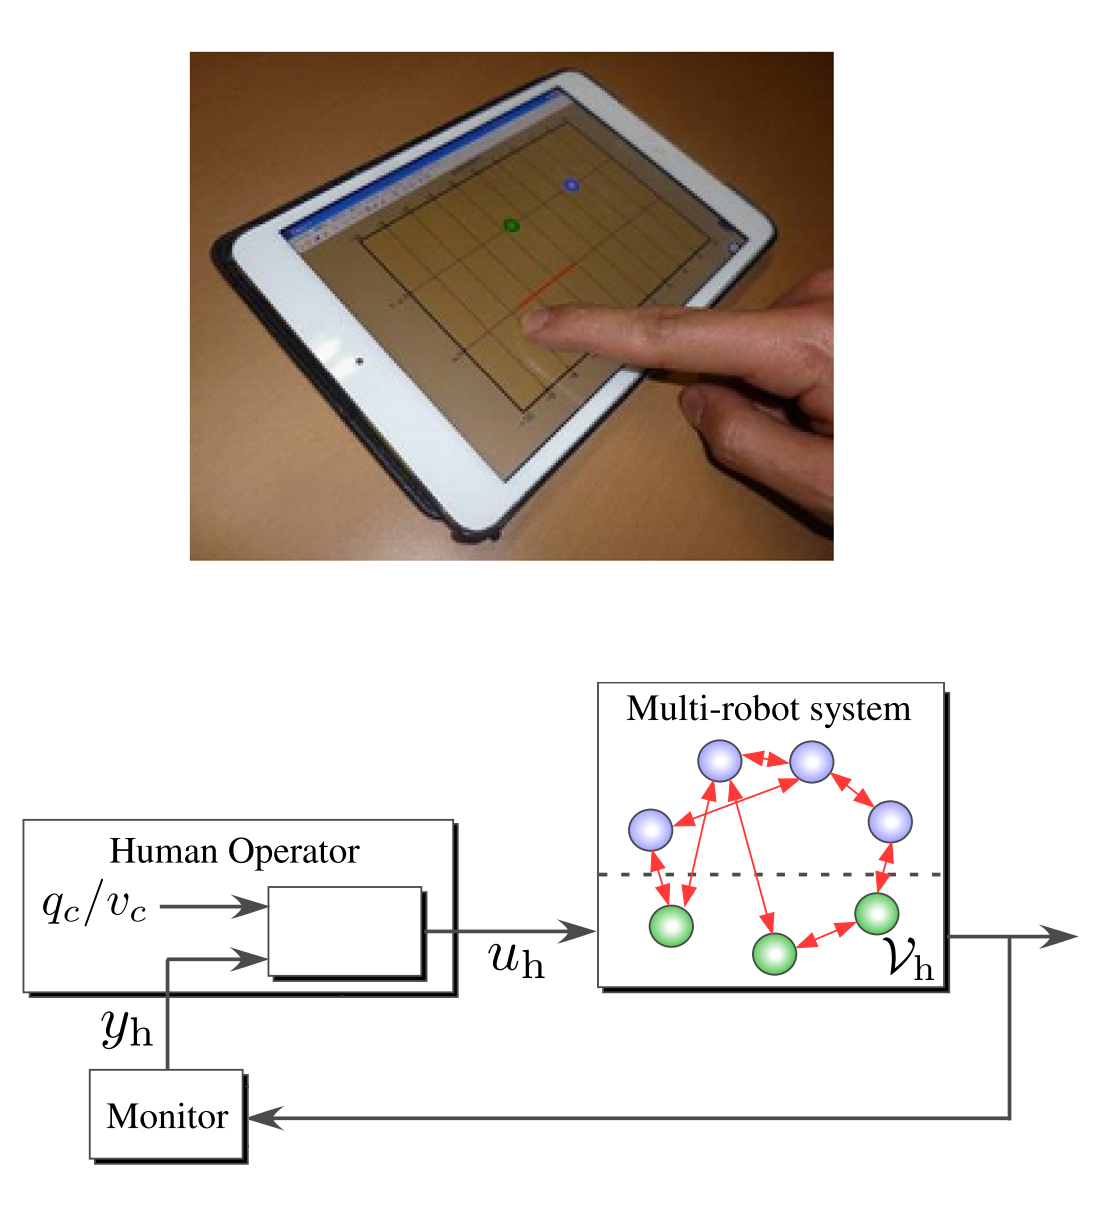
\includegraphics[width=1.1\textwidth]{HumanSwarmPres.png}			
			\end{figure}			
		\end{columns}
		

%\begin{table}
%	\centering
%	\small
%	%\caption[port-Hamiltonian system variables of mechanical elements]{port-Hamiltonian system variables of mechanical elements}\vspace{10pt}	
%	\begin{tabular}{ l | l | l | l }
%		& \textbf{Spring} & \textbf{Mass} & \textbf{Damper} \\ \hline
%		\textbf{Effort variable} & Wrench $W$ & Twist $T$ & Wrench $ W $ \\ \hline
%		\textbf{Flow variable} & Twist $ T $ & Wrench $ W $ & Twist $ T $ \\ \hline
%		\textbf{State variable} & Config. $H$ & Momentum $ P $ & - \\ \hline
%		\textbf{Energy function} & $ V_\g{P}(H) $ & $ V_\g{K} = \frac{1}{2}P^TM^{-1}P $ &$V_\g{D}^* =\frac{1}{2} T^TDT  $ \\ 
%	\end{tabular}
%\end{table}
			



\end{frame}


\section{Perception}

\begin{frame}
	\frametitle{Human Perception Resolution}
Passivation of delayed communication:
\begin{itemize}
\item Hard contacts are displayed softer
\item Telerobot seems to be more inert
\end{itemize}
Just noticeable difference (JND) for inertias: $21$\% and for stiffness $8$\%\\
Displayed impedances for free motion and hard contact
\[Z_\mathrm{m}^* = \frac{bT}{2} s \;\; , \;\; Z_\mathrm{k}^* = \frac{2k_eb}{2bk_e T}\frac{1}{s}
\]
Tuning the wave impedance gives conflictive results\\
Just not noticeable deviation in stiffness
\[b > (1-\text{JND}_k) \frac{k_e T}{2}\]
Perceived stiffness is not compromised, inertia display more realistic


\end{frame}


\section{Cognition}

\begin{frame}

	\frametitle{Unchanged behaviour: Zero-order hold}
	Shared control of quadruped robot: Human controls front legs \\
	Automatic positioning of rear legs to achieve
	\begin{itemize}
	\item Gait stability during rear leg change
	\item Gait stability for the next front leg steps
	\end{itemize}
	Prediction of next step allow for a large step size\\
	
\noindent{\color{tum_blue}\rule[0.5ex]{\linewidth}{1.5pt}}\vspace{-4pt}
	Zero-order hold extrapolation suitable for small prediction horizon\\
	User study: faster locomotion than least square system identification
	\begin{figure}
			\centering
			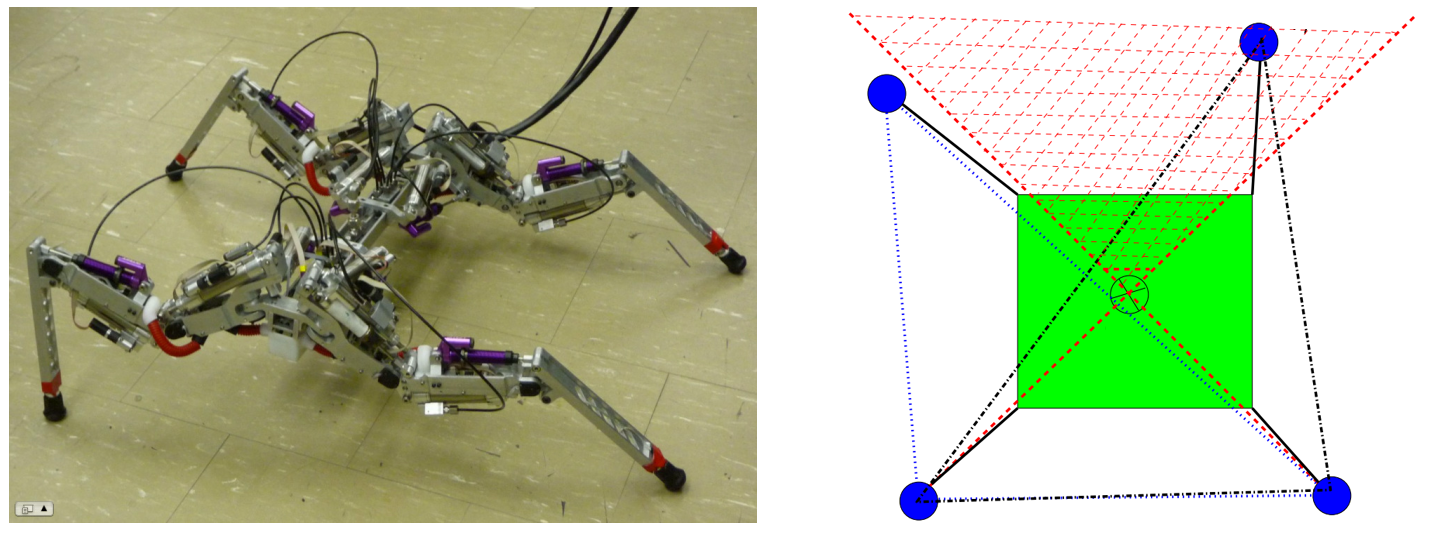
\includegraphics[width=0.7\textwidth]{4MPC.png}			
	\end{figure}
%	\begin{figure}
%		\flushleft
%		\footnotesize
%\begin{tikzpicture}
\begin{groupplot}[
      group style={group size=2 by 3,ylabels at=edge left},
      ylabel style={text height=0.02\textwidth,inner ysep=-5pt},
      grid=major,height=0.31\linewidth,width=0.5\linewidth,/tikz/font=\tiny
    ]
    \nextgroupplot[ylabel={Position $p_x$[m]}]
    \addplot[black,] table {../../plotdata/CaVitrans_desired position.txt}; 
	\addplot[blue,] table {../../plotdata/DIPCctrans_position.txt};
	\addplot[green,] table {../../plotdata/StrIPCtrans_position.txt};
	\addplot[red,] table {../../plotdata/CaVitrans_position.txt};
	\coordinate (top) at (rel axis cs:0,1);% coordinate at top of the first plot
	\nextgroupplot[ylabel={Orient. $\Phi_z$[rad]}]
	\addplot[black,] table {../../plotdata/CaVirot_desired Orientation.txt};
	\addplot[blue,] table {../../plotdata/DIPCcrot_Orientation.txt};
	\addplot[red,] table {../../plotdata/CaVirot_Orientation.txt};
	\addplot[green,] table {../../plotdata/StrIPCrot_Orientation.txt};
	\coordinate (bot) at (rel axis cs:1,0);% coordinate at bottom of the last plot
  \end{groupplot}
  % legend
  \path (top|-current bounding box.north)--
        coordinate(legendpos)
        (bot|-current bounding box.north);
  \matrix[
      matrix of nodes,
      anchor=south,
      draw,
      inner sep=0.2em,
    ]at([yshift=1ex]legendpos)
    {	{\color{black}\textemdash} &{desired traj.}&[3pt]
	    {\color{blue}\textemdash} &{constrained dIPC}&[3pt]
      {\color{red}\textemdash} &{impedance ctrl}&[3pt]
      {\color{green}\textemdash} &{dyn. IPC}&[3pt]\\};      
\end{tikzpicture} 
\begin{tikzpicture}
\hspace{3pt}
\begin{groupplot}[
      group style={group size=2 by 3,ylabels at=edge left},
      ylabel style={text height=0.02\textwidth,inner ysep=-5pt},
      grid=major,height=0.31\linewidth,width=0.5\linewidth,/tikz/font=\tiny
    ]
    \nextgroupplot[ylabel={Lin. vel. $\dot{p}_x$[m/s]}] 
    \addplot[black,] table {../../plotdata/CaVitrans_desired velocity.txt};
	\addplot[blue,] table {../../plotdata/DIPCctrans_Velocity.txt};
	\addplot[red,] table {../../plotdata/CaVitrans_Velocity.txt};
	\addplot[green,] table {../../plotdata/StrIPCtrans_Velocity.txt};
	\coordinate (top) at (rel axis cs:0,1);% coordinate at top of the first plot
	\nextgroupplot[ylabel={Ang. vel. $\omega_z$[rad/s]}]
	\addplot[black,] table {../../plotdata/CaVirot_desired ang velocity.txt};
	\addplot[blue,] table {../../plotdata/DIPCcrot_Angular Velocity.txt};
	\addplot[red,] table {../../plotdata/CaVirot_Angular Velocity.txt};
	\addplot[green,] table {../../plotdata/StrIPCrot_Angular Velocity.txt};
	\coordinate (bot) at (rel axis cs:1,0);% coordinate at bottom of the last plot
  \end{groupplot}
  % legend
%  \path (top|-current bounding box.north)--
%        coordinate(legendpos)
%        (bot|-current bounding box.north);
%  \matrix[
%      matrix of nodes,
%      anchor=south,
%      draw,
%      inner sep=0.2em,
%    ]at([yshift=1ex]legendpos)
%    { \ref*{plots:errVeloc}&{ $\Delta\dot{p}_x$ [m/s]}&[5pt]
%      \ref*{plots:errAngVel}&{ $\Delta\omega_z$ [rad/s]}&[5pt]\\};
\end{tikzpicture}
\begin{tikzpicture}
\begin{groupplot}[
	group style={group size=2 by 3,ylabels at=edge left},
	ylabel style={text height=0.02\textwidth,inner ysep=-10pt},
	grid=major,height=0.31\linewidth,width=0.5\linewidth,/tikz/font=\tiny
	]
	\nextgroupplot[xlabel={$t$[s]}, ylabel={Force $f_x$[N]}] 
	\addplot[blue,] table {../../plotdata/DIPCctrans_Manipulator wrench_tx.txt};
	\addplot[red,] table {../../plotdata/CaVitrans_Manipulator wrench_tx.txt};
	\addplot[green,] table {../../plotdata/StrIPCtrans_Manipulator wrench_tx.txt};
	\coordinate (top) at (rel axis cs:0,1);% coordinate at top of the first plot
	\nextgroupplot[xlabel={$t$[s]}, ylabel={Force $f_y$[N]}]
	\addplot[blue,] table {../../plotdata/DIPCcrot_Manipulator wrench_ty.txt};
	\addplot[red,] table {../../plotdata/CaVirot_Manipulator wrench_ty.txt};
	\addplot[green,] table {../../plotdata/StrIPCrot_Manipulator wrench_ty.txt};
	\coordinate (bot) at (rel axis cs:1,0);% coordinate at bottom of the last plot
\end{groupplot}
\end{tikzpicture} 

%\begin{tikzpicture}
%\begin{groupplot}[
%      group style={group size=2 by 3,ylabels at=edge 			left},
%      ylabel style={text height=0.02\textwidth,inner 			ysep=0pt},
%      grid=major,height=0.35\linewidth,width=0.495\linewidth,/tikz/font=\small
%    ]
%    \nextgroupplot[ylabel={Manipulator wrench}]  
%	\addplot[red,] table {../../plotdata/DIPCctrans_Manipulator wrench_tx.txt}; 
%	\addplot[blue,] table {../../plotdata/DIPCctrans_Manipulator wrench_ty.txt}; 
%	\addplot[green,] table {../../plotdata/DIPCctrans_Manipulator wrench_rz.txt};	
%	\coordinate (top) at (rel axis cs:0,1);% coordinate at top of the first plot
%	\nextgroupplot
%	\addplot[red,] table {../../plotdata/DIPCcrot_Manipulator wrench_tx.txt};\label{plots:forcex}
%	\addplot[blue,] table {../../plotdata/DIPCcrot_Manipulator wrench_ty.txt};\label{plots:forcey} 
%	\addplot[green,] table {../../plotdata/DIPCcrot_Manipulator wrench_rz.txt};\label{plots:torquez}	
%	\coordinate (bot) at (rel axis cs:1,0);% coordinate at bottom of the last plot
%  \end{groupplot}
%  % legend
%  \path (top|-current bounding box.north)--
%        coordinate(legendpos)
%        (bot|-current bounding box.north);
%  \matrix[
%      matrix of nodes,
%      anchor=south,
%      draw,
%      inner sep=0.2em,
%    ]at([yshift=1ex]legendpos)
%    { \ref*{plots:forcex}&{ $f_x$ [N]}&[5pt]
%    	  \ref*{plots:forcey}&{ $f_y$ [N]}&[5pt]
%      \ref*{plots:torquez}&{ $m_z$ [Nm]}&[5pt]\\};
%\end{tikzpicture}



%%\begin{tikzpicture}
\begin{groupplot}[
      group style={group size=2 by 3,ylabels at=edge 			left},
      ylabel style={text height=0.02\textwidth,inner 			ysep=-5pt},
      grid=major,height=0.3\linewidth,width=0.48\linewidth,/tikz/font=\tiny
    ]
    \nextgroupplot[ylabel={Position $\Delta p_x$[m]}] 
	\addplot[blue,] table {../../plotdata/DIPCctrans_errPos.txt};
	%\addplot[green,] table {../../plotdata/StrIPCtrans_errPos.txt};
	%\addplot[red,] table {../../plotdata/CaVitrans_errPos.txt};
	\coordinate (top) at (rel axis cs:0,1);% coordinate at top of the first plot
	\nextgroupplot[ylabel={Orient. $\Delta \Phi_z$[rad]}]
	\addplot[blue,] table {../../plotdata/DIPCcrot_errOrient.txt};
	%\addplot[red,] table {../../plotdata/CaVirot_errOrient.txt};
	%\addplot[green,] table {../../plotdata/StrIPCrot_errOrient.txt};
	\coordinate (bot) at (rel axis cs:1,0);% coordinate at bottom of the last plot
  \end{groupplot}
%  % legend
%  \path (top|-current bounding box.north)--
%        coordinate(legendpos)
%        (bot|-current bounding box.north);
%  \matrix[
%      matrix of nodes,
%      anchor=south,
%      draw,
%      inner sep=0.2em,
%    ]at([yshift=1ex]legendpos)
%    { {\color{blue}\textemdash} &{constrained IPC}&[3pt]
%      {\color{red}\textemdash} &{classic impedance control}&[3pt]
%      {\color{green}\textemdash} &{classic IPC}&[3pt]\\};
      
\end{tikzpicture} 



\begin{tikzpicture}
\begin{groupplot}[
      group style={group size=2 by 3,ylabels at=edge 			left},
      ylabel style={text height=0.02\textwidth,inner ysep=-5pt},
      grid=major,height=0.3\linewidth,width=0.48\linewidth, /tikz/font=\tiny ]
    \nextgroupplot[ylabel={Lin. vel. $\Delta \dot{p}_x$[m/s]}] 
	\addplot[blue,] table {../../plotdata/DIPCctrans_errVeloc.txt};
	%\addplot[red,] table {../../plotdata/CaVitrans_errVeloc.txt};
	%\addplot[green,] table {../../plotdata/StrIPCtrans_errVeloc.txt};
	\coordinate (top) at (rel axis cs:0,1);% coordinate at top of the first plot
	\nextgroupplot[ylabel={Ang. vel. $\Delta \omega_z$[rad/s]}]
	\addplot[blue,] table {../../plotdata/DIPCcrot_errAngVel.txt};
	%\addplot[red,] table {../../plotdata/CaVirot_errAngVel.txt};
	%\addplot[green,] table {../../plotdata/StrIPCrot_errAngVel.txt};
	\coordinate (bot) at (rel axis cs:1,0);% coordinate at bottom of the last plot
  \end{groupplot}
  % legend
%  \path (top|-current bounding box.north)--
%        coordinate(legendpos)
%        (bot|-current bounding box.north);
%  \matrix[
%      matrix of nodes,
%      anchor=south,
%      draw,
%      inner sep=0.2em,
%    ]at([yshift=1ex]legendpos)
%    { \ref*{plots:errVeloc}&{ $\Delta\dot{p}_x$ [m/s]}&[5pt]
%      \ref*{plots:errAngVel}&{ $\Delta\omega_z$ [rad/s]}&[5pt]\\};
\end{tikzpicture} 



\begin{tikzpicture}
\begin{groupplot}[
      group style={group size=2 by 3,ylabels at=edge 			left},
      ylabel style={text height=0.02\textwidth,inner 			ysep=-5pt},
      grid=major,height=0.3\linewidth,width=0.48\linewidth,/tikz/font=\tiny
    ]
    \nextgroupplot[xlabel={$t$[s]},ylabel={Wrench $f_x$[N]}]  
	\addplot[red,] table {../../plotdata/DIPCctrans_Manipulator wrench_tx.txt}; 
	\addplot[blue,] table {../../plotdata/DIPCctrans_Manipulator wrench_ty.txt}; 
	\addplot[green,] table {../../plotdata/DIPCctrans_Manipulator wrench_rz.txt};	
	\coordinate (top) at (rel axis cs:0,1);% coordinate at top of the first plot
	\nextgroupplot[xlabel={$t$[s]},ylabel={$f_x$[N],$f_y$[N],$m_z$[Nm]}]
	\addplot[red,] table {../../plotdata/DIPCcrot_Manipulator wrench_tx.txt};\label{plots:forcex}
	\addplot[blue,] table {../../plotdata/DIPCcrot_Manipulator wrench_ty.txt};\label{plots:forcey} 
	\addplot[green,] table {../../plotdata/DIPCcrot_Manipulator wrench_rz.txt};\label{plots:torquez}	
	\coordinate (bot) at (rel axis cs:1,0);% coordinate at bottom of the last plot
  \end{groupplot}
%  % legend
%  \path (top|-current bounding box.north)--
%        coordinate(legendpos)
%        (bot|-current bounding box.north);
%  \matrix[
%      matrix of nodes,
%      anchor=south,
%      draw,
%      inner sep=0.2em,
%    ]at([yshift=1ex]legendpos)
%    { \ref*{plots:forcex}&{ $f_x$ [N]}&[5pt]
%    	  \ref*{plots:forcey}&{ $f_y$ [N]}&[5pt]
%      \ref*{plots:torquez}&{ $m_z$ [Nm]}&[5pt]\\};
\end{tikzpicture}



%\end{figure}
\end{frame}


%\begin{frame}
%	\frametitle{Trajectory tracking: Classic (enhanced) IPC }
%	\frametitle{Trajectory tracking: Comparison}
%	\vspace{-30pt}
%	\begin{figure}
%%\begin{tikzpicture}
\begin{groupplot}[
      group style={group size=2 by 3,ylabels at=edge left},
      ylabel style={text height=0.02\textwidth,inner ysep=-5pt},
      grid=major,height=0.31\linewidth,width=0.5\linewidth,/tikz/font=\tiny
    ]
    \nextgroupplot[ylabel={Position $p_x$[m]}]
    \addplot[black,] table {../../plotdata/CaVitrans_desired position.txt}; 
	\addplot[blue,] table {../../plotdata/DIPCctrans_position.txt};
	\addplot[green,] table {../../plotdata/StrIPCtrans_position.txt};
	\addplot[red,] table {../../plotdata/CaVitrans_position.txt};
	\coordinate (top) at (rel axis cs:0,1);% coordinate at top of the first plot
	\nextgroupplot[ylabel={Orient. $\Phi_z$[rad]}]
	\addplot[black,] table {../../plotdata/CaVirot_desired Orientation.txt};
	\addplot[blue,] table {../../plotdata/DIPCcrot_Orientation.txt};
	\addplot[red,] table {../../plotdata/CaVirot_Orientation.txt};
	\addplot[green,] table {../../plotdata/StrIPCrot_Orientation.txt};
	\coordinate (bot) at (rel axis cs:1,0);% coordinate at bottom of the last plot
  \end{groupplot}
  % legend
  \path (top|-current bounding box.north)--
        coordinate(legendpos)
        (bot|-current bounding box.north);
  \matrix[
      matrix of nodes,
      anchor=south,
      draw,
      inner sep=0.2em,
    ]at([yshift=1ex]legendpos)
    {	{\color{black}\textemdash} &{desired traj.}&[3pt]
	    {\color{blue}\textemdash} &{constrained dIPC}&[3pt]
      {\color{red}\textemdash} &{impedance ctrl}&[3pt]
      {\color{green}\textemdash} &{dyn. IPC}&[3pt]\\};      
\end{tikzpicture} 
\begin{tikzpicture}
\hspace{3pt}
\begin{groupplot}[
      group style={group size=2 by 3,ylabels at=edge left},
      ylabel style={text height=0.02\textwidth,inner ysep=-5pt},
      grid=major,height=0.31\linewidth,width=0.5\linewidth,/tikz/font=\tiny
    ]
    \nextgroupplot[ylabel={Lin. vel. $\dot{p}_x$[m/s]}] 
    \addplot[black,] table {../../plotdata/CaVitrans_desired velocity.txt};
	\addplot[blue,] table {../../plotdata/DIPCctrans_Velocity.txt};
	\addplot[red,] table {../../plotdata/CaVitrans_Velocity.txt};
	\addplot[green,] table {../../plotdata/StrIPCtrans_Velocity.txt};
	\coordinate (top) at (rel axis cs:0,1);% coordinate at top of the first plot
	\nextgroupplot[ylabel={Ang. vel. $\omega_z$[rad/s]}]
	\addplot[black,] table {../../plotdata/CaVirot_desired ang velocity.txt};
	\addplot[blue,] table {../../plotdata/DIPCcrot_Angular Velocity.txt};
	\addplot[red,] table {../../plotdata/CaVirot_Angular Velocity.txt};
	\addplot[green,] table {../../plotdata/StrIPCrot_Angular Velocity.txt};
	\coordinate (bot) at (rel axis cs:1,0);% coordinate at bottom of the last plot
  \end{groupplot}
  % legend
%  \path (top|-current bounding box.north)--
%        coordinate(legendpos)
%        (bot|-current bounding box.north);
%  \matrix[
%      matrix of nodes,
%      anchor=south,
%      draw,
%      inner sep=0.2em,
%    ]at([yshift=1ex]legendpos)
%    { \ref*{plots:errVeloc}&{ $\Delta\dot{p}_x$ [m/s]}&[5pt]
%      \ref*{plots:errAngVel}&{ $\Delta\omega_z$ [rad/s]}&[5pt]\\};
\end{tikzpicture}
\begin{tikzpicture}
\begin{groupplot}[
	group style={group size=2 by 3,ylabels at=edge left},
	ylabel style={text height=0.02\textwidth,inner ysep=-10pt},
	grid=major,height=0.31\linewidth,width=0.5\linewidth,/tikz/font=\tiny
	]
	\nextgroupplot[xlabel={$t$[s]}, ylabel={Force $f_x$[N]}] 
	\addplot[blue,] table {../../plotdata/DIPCctrans_Manipulator wrench_tx.txt};
	\addplot[red,] table {../../plotdata/CaVitrans_Manipulator wrench_tx.txt};
	\addplot[green,] table {../../plotdata/StrIPCtrans_Manipulator wrench_tx.txt};
	\coordinate (top) at (rel axis cs:0,1);% coordinate at top of the first plot
	\nextgroupplot[xlabel={$t$[s]}, ylabel={Force $f_y$[N]}]
	\addplot[blue,] table {../../plotdata/DIPCcrot_Manipulator wrench_ty.txt};
	\addplot[red,] table {../../plotdata/CaVirot_Manipulator wrench_ty.txt};
	\addplot[green,] table {../../plotdata/StrIPCrot_Manipulator wrench_ty.txt};
	\coordinate (bot) at (rel axis cs:1,0);% coordinate at bottom of the last plot
\end{groupplot}
\end{tikzpicture} 

%\begin{tikzpicture}
%\begin{groupplot}[
%      group style={group size=2 by 3,ylabels at=edge 			left},
%      ylabel style={text height=0.02\textwidth,inner 			ysep=0pt},
%      grid=major,height=0.35\linewidth,width=0.495\linewidth,/tikz/font=\small
%    ]
%    \nextgroupplot[ylabel={Manipulator wrench}]  
%	\addplot[red,] table {../../plotdata/DIPCctrans_Manipulator wrench_tx.txt}; 
%	\addplot[blue,] table {../../plotdata/DIPCctrans_Manipulator wrench_ty.txt}; 
%	\addplot[green,] table {../../plotdata/DIPCctrans_Manipulator wrench_rz.txt};	
%	\coordinate (top) at (rel axis cs:0,1);% coordinate at top of the first plot
%	\nextgroupplot
%	\addplot[red,] table {../../plotdata/DIPCcrot_Manipulator wrench_tx.txt};\label{plots:forcex}
%	\addplot[blue,] table {../../plotdata/DIPCcrot_Manipulator wrench_ty.txt};\label{plots:forcey} 
%	\addplot[green,] table {../../plotdata/DIPCcrot_Manipulator wrench_rz.txt};\label{plots:torquez}	
%	\coordinate (bot) at (rel axis cs:1,0);% coordinate at bottom of the last plot
%  \end{groupplot}
%  % legend
%  \path (top|-current bounding box.north)--
%        coordinate(legendpos)
%        (bot|-current bounding box.north);
%  \matrix[
%      matrix of nodes,
%      anchor=south,
%      draw,
%      inner sep=0.2em,
%    ]at([yshift=1ex]legendpos)
%    { \ref*{plots:forcex}&{ $f_x$ [N]}&[5pt]
%    	  \ref*{plots:forcey}&{ $f_y$ [N]}&[5pt]
%      \ref*{plots:torquez}&{ $m_z$ [Nm]}&[5pt]\\};
%\end{tikzpicture}



%\begin{tikzpicture}
\begin{groupplot}[
      group style={group size=2 by 3,ylabels at=edge 			left},
      ylabel style={text height=0.02\textwidth,inner 			ysep=-5pt},
      grid=major,height=0.3\linewidth,width=0.48\linewidth,/tikz/font=\tiny
    ]
    \nextgroupplot[ylabel={Position $\Delta p_x$[m]}] 
	%\addplot[blue,] table {../../plotdata/DIPCctrans_errPos.txt};
	\addplot[blue,] table {../../plotdata/StrIPCtrans_errPos.txt};
	%\addplot[red,] table {../../plotdata/CaVitrans_errPos.txt};
	\coordinate (top) at (rel axis cs:0,1);% coordinate at top of the first plot
	\nextgroupplot[ylabel={Orient. $\Delta \Phi_z$[rad]}]
	%\addplot[blue,] table {../../plotdata/DIPCcrot_errOrient.txt};
	%\addplot[red,] table {../../plotdata/CaVirot_errOrient.txt};
	\addplot[blue,] table {../../plotdata/StrIPCrot_errOrient.txt};
	\coordinate (bot) at (rel axis cs:1,0);% coordinate at bottom of the last plot
  \end{groupplot}
%  % legend
%  \path (top|-current bounding box.north)--
%        coordinate(legendpos)
%        (bot|-current bounding box.north);
%  \matrix[
%      matrix of nodes,
%      anchor=south,
%      draw,
%      inner sep=0.2em,
%    ]at([yshift=1ex]legendpos)
%    { {\color{blue}\textemdash} &{constrained IPC}&[3pt]
%      {\color{red}\textemdash} &{classic impedance control}&[3pt]
%      {\color{green}\textemdash} &{classic IPC}&[3pt]\\};
      
\end{tikzpicture} 



\begin{tikzpicture}
\begin{groupplot}[
      group style={group size=2 by 3,ylabels at=edge 			left},
      ylabel style={text height=0.02\textwidth,inner ysep=-5pt},
      grid=major,height=0.3\linewidth,width=0.48\linewidth, /tikz/font=\tiny ]
    \nextgroupplot[ylabel={Lin. vel. $\Delta \dot{p}_x$[m/s]}] 
	%\addplot[blue,] table {../../plotdata/DIPCctrans_errVeloc.txt};
	%\addplot[red,] table {../../plotdata/CaVitrans_errVeloc.txt};
	\addplot[blue,] table {../../plotdata/StrIPCtrans_errVeloc.txt};
	\coordinate (top) at (rel axis cs:0,1);% coordinate at top of the first plot
	\nextgroupplot[ylabel={Ang. vel. $\Delta \omega_z$[rad/s]}]
	%\addplot[blue,] table {../../plotdata/DIPCcrot_errAngVel.txt};
	%\addplot[red,] table {../../plotdata/CaVirot_errAngVel.txt};
	\addplot[blue,] table {../../plotdata/StrIPCrot_errAngVel.txt};
	\coordinate (bot) at (rel axis cs:1,0);% coordinate at bottom of the last plot
  \end{groupplot}
  % legend
%  \path (top|-current bounding box.north)--
%        coordinate(legendpos)
%        (bot|-current bounding box.north);
%  \matrix[
%      matrix of nodes,
%      anchor=south,
%      draw,
%      inner sep=0.2em,
%    ]at([yshift=1ex]legendpos)
%    { \ref*{plots:errVeloc}&{ $\Delta\dot{p}_x$ [m/s]}&[5pt]
%      \ref*{plots:errAngVel}&{ $\Delta\omega_z$ [rad/s]}&[5pt]\\};
\end{tikzpicture} 



\begin{tikzpicture}
\begin{groupplot}[
      group style={group size=2 by 3,ylabels at=edge 			left},
      ylabel style={text height=0.02\textwidth,inner 			ysep=-5pt},
      grid=major,height=0.3\linewidth,width=0.48\linewidth,/tikz/font=\tiny
    ]
    \nextgroupplot[xlabel={$t$[s]},ylabel={Wrench $f_x$[N]}]  
	\addplot[red,] table {../../plotdata/StrIPCtrans_Manipulator wrench_tx.txt}; 
	\addplot[blue,] table {../../plotdata/StrIPCtrans_Manipulator wrench_ty.txt}; 
	\addplot[green,] table {../../plotdata/StrIPCtrans_Manipulator wrench_rz.txt};	
	\coordinate (top) at (rel axis cs:0,1);% coordinate at top of the first plot
	\nextgroupplot[xlabel={$t$[s]},ylabel={$f_x$[N],$f_y$[N],$m_z$[Nm]}]
	\addplot[red,] table {../../plotdata/StrIPCrot_Manipulator wrench_tx.txt};\label{plots:forcex}
	\addplot[blue,] table {../../plotdata/StrIPCrot_Manipulator wrench_ty.txt};\label{plots:forcey} 
	\addplot[green,] table {../../plotdata/StrIPCrot_Manipulator wrench_rz.txt};\label{plots:torquez}	
	\coordinate (bot) at (rel axis cs:1,0);% coordinate at bottom of the last plot
  \end{groupplot}
%  % legend
%  \path (top|-current bounding box.north)--
%        coordinate(legendpos)
%        (bot|-current bounding box.north);
%  \matrix[
%      matrix of nodes,
%      anchor=south,
%      draw,
%      inner sep=0.2em,
%    ]at([yshift=1ex]legendpos)
%    { \ref*{plots:forcex}&{ $f_x$ [N]}&[5pt]
%    	  \ref*{plots:forcey}&{ $f_y$ [N]}&[5pt]
%      \ref*{plots:torquez}&{ $m_z$ [Nm]}&[5pt]\\};
\end{tikzpicture}



%\end{figure}
%\end{frame}




\begin{frame}
	\frametitle{Human motion sequence learning}
{\small Faultless execution of fine manipulation tasks in space \\
Traded control: robot automatically executes repetitive tasks\\
Learning "good" motion sequences by demonstration\\
Human motion is a doubly stochastic process: Hidden Markov Models\\
States (intention) are estimated from the observations (motion)\\
Selection of the best learned trajectory 
\[
\max P(\lambda_r \mid O^*) = \frac{P(O^* \mid \lambda_r) P(\lambda_r)}{P(O*)} \; , \; \forall r=1...R
\]
Elimination of minor uncertainties, Trading of control not perceivable}
			\begin{figure}
			\centering
			\tiny
			%\psfrag{q1}[Bl][Bl]{\small $\alpha$}
			\def\svgwidth{0.8\columnwidth}
			\input{HiddenMarkov.eps_tex}								
			\end{figure}	 
	
	
\end{frame}

\begin{frame}
	\frametitle{Forced-choice decision making}
	{\normalsize
Supervision of multiple surveillance agents\\
Pre-selection and scheduling of data to evaluate\\
Modelling of human decision making for incident identification and estimation of the evaluation time\\
Two alternative forced choice by evidence accumulation\\
Drift diffusion model
\[
dx(t) = \mu dt + \sigma dW(t),
\]}
 	\begin{figure}
			\centering
			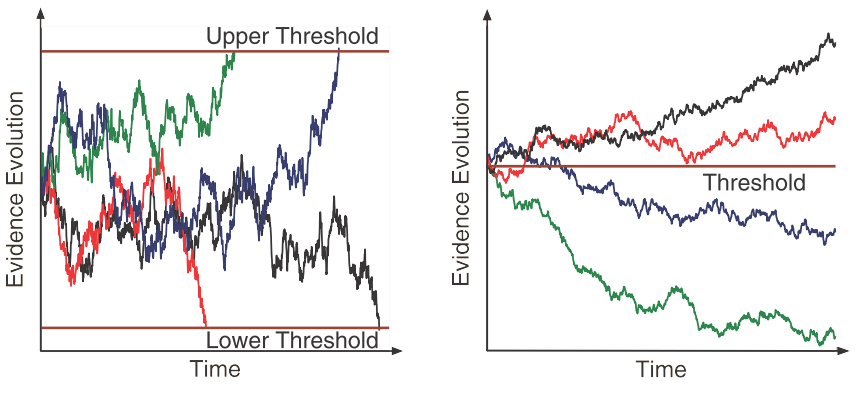
\includegraphics[width=0.7\textwidth]{EvidenceAcc.png}			
	\end{figure}
	 
	
	
\end{frame}

%\begin{frame}
%	\frametitle{Comparison: internal forces (rotation)}
%\begin{figure}[t]
%
%\begin{tikzpicture}
%	\begin{axis} [
%		ylabel = {f[N],m[Nm]},
%		xlabel = {t[s]},
%		minor y tick num = 1,
%		axis lines = left,
%		%legend entries = {force $f_{int,x}$, force $f_{int,y}$, torque $m_{int,z}$},
%		%legend style = {at={(axis cs:2.6, 0.04)}, anchor = north},
%		%legend cell align=left,
%		grid = major,
%		height=3.3cm,
%		width=0.98\linewidth
%	]
%\addplot[red,]
%	table {/home/mangerer/MAgit/MA/Latex/plotdata/DePaIntWrenchtx.txt};
%\addplot[blue,]
%	table {/home/mangerer/MAgit/MA/Latex/plotdata/DePaIntWrenchty.txt};
%	\addplot[green,]
%	table {/home/mangerer/MAgit/MA/Latex/plotdata/DePaIntWrenchrz.txt};\end{axis}
%\end{tikzpicture}
%\begin{tikzpicture}
%	\begin{axis} [
%		ylabel = {f[N],m[Nm]},
%		xlabel = {t[s]},
%		minor y tick num = 1,
%		axis lines = left,
%		legend entries = {force $f_{int,x}$, force $f_{int,y}$, torque $m_{int,z}$},
%		legend style = {at={(axis cs:2.6, 0.1)}, anchor = north},
%		legend cell align=left,
%		grid = major,
%		height=3.3cm,
%		width=0.98\linewidth
%	]
%\addplot[red,]
%	table {/home/mangerer/MAgit/MA/Latex/plotdata/DIPCInternalWrenchtx.txt};
%\addplot[blue,]
%	table {/home/mangerer/MAgit/MA/Latex/plotdata/DIPCInternalWrenchty.txt};
%	\addplot[green,]
%	table {/home/mangerer/MAgit/MA/Latex/plotdata/DIPCInternalWrenchrz.txt};\end{axis}
%\end{tikzpicture}
%\vspace{-28pt}
%\caption{Top: Object force feed-forward;
%Bottom: Virtual Object}
%\end{figure}
%\end{frame}
\section{Conclusion}


\begin{frame}
	\frametitle{Conclusion}

\vspace{6pt}
{\color{tum_blue}\textbf{Human modelling in teleoperation can}}\vspace{-6pt}
\noindent{\color{tum_blue}\rule[0.5ex]{\linewidth}{1.5pt}}
	\begin{itemize}
	\item ensure stability with the human in the loop
	\item support decision making 
	\item improve manipulation skill
	\end{itemize}
\end{frame}
\appendix

\begin{frame}[allowframebreaks]
	\frametitle{References}
	%\tiny
	%\bibliographystyle{plain}
	%\bibliography{ref}
	\printbibliography
\end{frame}

%\begin{frame}
%	%\frametitle{Trajectory tracking: Constrained dynamic IPC }
%	\frametitle{{\tiny Backup} Trajectory tracking: Comparison}
%	\vspace{-30pt}
%	\begin{figure}
%		\centering
%		\begin{tikzpicture}
\hspace{10pt}
\begin{groupplot}[
      group style={group size=2 by 3,ylabels at=edge 			left},
      ylabel style={text height=0.02\textwidth,inner 			ysep=-5pt},
      grid=major,height=0.35\linewidth,width=0.5\linewidth,/tikz/font=\footnotesize
    ]
    \nextgroupplot[ylabel={Position $\Delta p_x$[m]}] 
	\addplot[blue,] table {../../plotdata/DIPCctrans_errPos.txt};
	\addplot[green,] table {../../plotdata/StrIPCtrans_errPos.txt};
	\addplot[red,] table {../../plotdata/CaVitrans_errPos.txt};
	\coordinate (top) at (rel axis cs:0,1);% coordinate at top of the first plot
	\nextgroupplot[ylabel={Orient. $\Delta \Phi_z$[rad]}]
	\addplot[blue,] table {../../plotdata/DIPCcrot_errOrient.txt};
	\addplot[red,] table {../../plotdata/CaVirot_errOrient.txt};
	\addplot[green,] table {../../plotdata/StrIPCrot_errOrient.txt};
	\coordinate (bot) at (rel axis cs:1,0);% coordinate at bottom of the last plot
  \end{groupplot}
  % legend
  \path (top|-current bounding box.north)--
        coordinate(legendpos)
        (bot|-current bounding box.north);
  \matrix[
      matrix of nodes,
      anchor=south,
      draw,
      inner sep=0.2em,
    ]at([yshift=1ex]legendpos)
    { {\color{blue}\textemdash} &{constrained dIPC}&[3pt]
      {\color{red}\textemdash} &{impedance control}&[3pt]
      {\color{green}\textemdash} &{dynamic IPC}&[3pt]\\};
      
\end{tikzpicture} 



\begin{tikzpicture}
\begin{groupplot}[
      group style={group size=2 by 3,ylabels at=edge 			left},
      ylabel style={text height=0.02\textwidth,inner ysep=-5pt},
      grid=major,height=0.35\linewidth,width=0.5\linewidth,/tikz/font=\footnotesize
    ]
    \nextgroupplot[xlabel={$t$[s]}, ylabel={Lin. vel. $\Delta \dot{p}_x$[m/s]}] 
	\addplot[blue,] table {../../plotdata/DIPCctrans_errVeloc.txt};
	\addplot[red,] table {../../plotdata/CaVitrans_errVeloc.txt};
	\addplot[green,] table {../../plotdata/StrIPCtrans_errVeloc.txt};
	\coordinate (top) at (rel axis cs:0,1);% coordinate at top of the first plot
	\nextgroupplot[xlabel={$t$[s]}, ylabel={Ang. vel. $\Delta \omega_z$[rad/s]}]
	\addplot[blue,] table {../../plotdata/DIPCcrot_errAngVel.txt};
	\addplot[red,] table {../../plotdata/CaVirot_errAngVel.txt};
	\addplot[green,] table {../../plotdata/StrIPCrot_errAngVel.txt};
	\coordinate (bot) at (rel axis cs:1,0);% coordinate at bottom of the last plot
  \end{groupplot}
  % legend
%  \path (top|-current bounding box.north)--
%        coordinate(legendpos)
%        (bot|-current bounding box.north);
%  \matrix[
%      matrix of nodes,
%      anchor=south,
%      draw,
%      inner sep=0.2em,
%    ]at([yshift=1ex]legendpos)
%    { \ref*{plots:errVeloc}&{ $\Delta\dot{p}_x$ [m/s]}&[5pt]
%      \ref*{plots:errAngVel}&{ $\Delta\omega_z$ [rad/s]}&[5pt]\\};
\end{tikzpicture} 
%		%\begin{tikzpicture}
\begin{groupplot}[
      group style={group size=2 by 3,ylabels at=edge 			left},
      ylabel style={text height=0.02\textwidth,inner 			ysep=-5pt},
      grid=major,height=0.3\linewidth,width=0.48\linewidth,/tikz/font=\tiny
    ]
    \nextgroupplot[ylabel={Position $\Delta p_x$[m]}] 
	\addplot[blue,] table {../../plotdata/DIPCctrans_errPos.txt};
	%\addplot[green,] table {../../plotdata/StrIPCtrans_errPos.txt};
	%\addplot[red,] table {../../plotdata/CaVitrans_errPos.txt};
	\coordinate (top) at (rel axis cs:0,1);% coordinate at top of the first plot
	\nextgroupplot[ylabel={Orient. $\Delta \Phi_z$[rad]}]
	\addplot[blue,] table {../../plotdata/DIPCcrot_errOrient.txt};
	%\addplot[red,] table {../../plotdata/CaVirot_errOrient.txt};
	%\addplot[green,] table {../../plotdata/StrIPCrot_errOrient.txt};
	\coordinate (bot) at (rel axis cs:1,0);% coordinate at bottom of the last plot
  \end{groupplot}
%  % legend
%  \path (top|-current bounding box.north)--
%        coordinate(legendpos)
%        (bot|-current bounding box.north);
%  \matrix[
%      matrix of nodes,
%      anchor=south,
%      draw,
%      inner sep=0.2em,
%    ]at([yshift=1ex]legendpos)
%    { {\color{blue}\textemdash} &{constrained IPC}&[3pt]
%      {\color{red}\textemdash} &{classic impedance control}&[3pt]
%      {\color{green}\textemdash} &{classic IPC}&[3pt]\\};
      
\end{tikzpicture} 



\begin{tikzpicture}
\begin{groupplot}[
      group style={group size=2 by 3,ylabels at=edge 			left},
      ylabel style={text height=0.02\textwidth,inner ysep=-5pt},
      grid=major,height=0.3\linewidth,width=0.48\linewidth, /tikz/font=\tiny ]
    \nextgroupplot[ylabel={Lin. vel. $\Delta \dot{p}_x$[m/s]}] 
	\addplot[blue,] table {../../plotdata/DIPCctrans_errVeloc.txt};
	%\addplot[red,] table {../../plotdata/CaVitrans_errVeloc.txt};
	%\addplot[green,] table {../../plotdata/StrIPCtrans_errVeloc.txt};
	\coordinate (top) at (rel axis cs:0,1);% coordinate at top of the first plot
	\nextgroupplot[ylabel={Ang. vel. $\Delta \omega_z$[rad/s]}]
	\addplot[blue,] table {../../plotdata/DIPCcrot_errAngVel.txt};
	%\addplot[red,] table {../../plotdata/CaVirot_errAngVel.txt};
	%\addplot[green,] table {../../plotdata/StrIPCrot_errAngVel.txt};
	\coordinate (bot) at (rel axis cs:1,0);% coordinate at bottom of the last plot
  \end{groupplot}
  % legend
%  \path (top|-current bounding box.north)--
%        coordinate(legendpos)
%        (bot|-current bounding box.north);
%  \matrix[
%      matrix of nodes,
%      anchor=south,
%      draw,
%      inner sep=0.2em,
%    ]at([yshift=1ex]legendpos)
%    { \ref*{plots:errVeloc}&{ $\Delta\dot{p}_x$ [m/s]}&[5pt]
%      \ref*{plots:errAngVel}&{ $\Delta\omega_z$ [rad/s]}&[5pt]\\};
\end{tikzpicture} 



\begin{tikzpicture}
\begin{groupplot}[
      group style={group size=2 by 3,ylabels at=edge 			left},
      ylabel style={text height=0.02\textwidth,inner 			ysep=-5pt},
      grid=major,height=0.3\linewidth,width=0.48\linewidth,/tikz/font=\tiny
    ]
    \nextgroupplot[xlabel={$t$[s]},ylabel={Wrench $f_x$[N]}]  
	\addplot[red,] table {../../plotdata/DIPCctrans_Manipulator wrench_tx.txt}; 
	\addplot[blue,] table {../../plotdata/DIPCctrans_Manipulator wrench_ty.txt}; 
	\addplot[green,] table {../../plotdata/DIPCctrans_Manipulator wrench_rz.txt};	
	\coordinate (top) at (rel axis cs:0,1);% coordinate at top of the first plot
	\nextgroupplot[xlabel={$t$[s]},ylabel={$f_x$[N],$f_y$[N],$m_z$[Nm]}]
	\addplot[red,] table {../../plotdata/DIPCcrot_Manipulator wrench_tx.txt};\label{plots:forcex}
	\addplot[blue,] table {../../plotdata/DIPCcrot_Manipulator wrench_ty.txt};\label{plots:forcey} 
	\addplot[green,] table {../../plotdata/DIPCcrot_Manipulator wrench_rz.txt};\label{plots:torquez}	
	\coordinate (bot) at (rel axis cs:1,0);% coordinate at bottom of the last plot
  \end{groupplot}
%  % legend
%  \path (top|-current bounding box.north)--
%        coordinate(legendpos)
%        (bot|-current bounding box.north);
%  \matrix[
%      matrix of nodes,
%      anchor=south,
%      draw,
%      inner sep=0.2em,
%    ]at([yshift=1ex]legendpos)
%    { \ref*{plots:forcex}&{ $f_x$ [N]}&[5pt]
%    	  \ref*{plots:forcey}&{ $f_y$ [N]}&[5pt]
%      \ref*{plots:torquez}&{ $m_z$ [Nm]}&[5pt]\\};
\end{tikzpicture}



%	\end{figure}
%\end{frame}
%
%\begin{frame}
%	\frametitle{{\tiny Backup} Trajectory tracking: Interpretation}
%	\begin{figure}
%		\centering
%		\small
%		\def\svgwidth{1\columnwidth}
%		\input{pics/ImpedanceIPC.eps_tex}
%	\end{figure}
%	Different role of inertias in the controllers: force gradients cause performance gap
%	\begin{figure}
%		\vspace{-30pt}
%		\begin{tikzpicture}
\begin{groupplot}[
      group style={group size=2 by 3,ylabels at=edge 			left},
      ylabel style={text height=0.02\textwidth,inner 			ysep=-5pt},
      grid=major,height=0.35\linewidth,width=0.48\linewidth,/tikz/font=\footnotesize
    ]
    \nextgroupplot[xlabel={$t$[s]}, ylabel={Force $f_x$[N]}] 
	\addplot[blue,] table {../../plotdata/DIPCctrans_Manipulator wrench_tx.txt};
	\addplot[red,] table {../../plotdata/CaVitrans_Manipulator wrench_tx.txt};
	\coordinate (top) at (rel axis cs:0,1);% coordinate at top of the first plot
	\nextgroupplot[xlabel={$t$[s]}, ylabel={Force $f_y$[N]}]
	\addplot[blue,] table {../../plotdata/DIPCcrot_Manipulator wrench_ty.txt};
	\addplot[red,] table {../../plotdata/CaVirot_Manipulator wrench_ty.txt};
	\coordinate (bot) at (rel axis cs:1,0);% coordinate at bottom of the last plot
  \end{groupplot}
  % legend
  \path (top|-current bounding box.north)--
        coordinate(legendpos)
        (bot|-current bounding box.north);
  \matrix[
      matrix of nodes,
      anchor=south,
      draw,
      inner sep=0.2em,
    ]at([yshift=1ex]legendpos)
    { {\color{blue}\textemdash} &{ constrained IPC}&[5pt]
      {\color{red}\textemdash} &{ classic impedance control}&[5pt]\\};
\end{tikzpicture}
%	\end{figure}
%\end{frame}

\end{document}
